\documentclass{article}
\usepackage{tipa}
\usepackage{tikz}
\usepackage{multirow,multicol}
\usetikzlibrary{shapes.geometric}

\newcommand{\ti}{\textipa}

%TODO fix table formatting to be side-by-side

\begin{document}

\section{Case Endings}

\begin{center}
\begin{tabular}{c| c c c}
  & \textbf{Sg} & \textbf{Pc} & \textbf{Pl} \\
  \hline
\textbf{NOM} & --\O & --ll\$ & --\O\textipa{:} \\
\textbf{ACC} & --l\$ & --ll\$ & --l\$n \\
\textbf{GEN} & --j & --j\$ll\$ & --j\$n \\
\textbf{LOC} & --t & --d\$ll\$  &--d\$n \\
\textbf{ABL} & --x & --ll\$x & --x\$n \\
\textbf{ALL} & --z & --ll\$z & --z\$n \\
\textbf{INS} & --r & --ll\$r & --r\$n \\
\textbf{VOC} & --k & \multicolumn{2}{c}{--k\$la} \\


\end{tabular}

\end{center}


\section{Definite Article}
\begin{center}
\begin{tabular}{c| c c c }
& \textbf{Sg} & \textbf{Pc} & \textbf{Pl} \\
\hline
\textbf{C1} & re & rex & ren \\
\textbf{C2} & ye & yeve & yen \\
\textbf{C3} & xi & xe & xen \\
\textbf{C4} & pse & psen & ox
\end{tabular}
\end{center}


\section{Subject Affixes}

\subsection{Aorist}
\begin{center}

\begin{tabular}{c| c c }
  & \textbf{Sg} & \textbf{Pc/Pl} \\
  \hline
  \textbf{1p} & --n & --m \\
  \textbf{2p}& --ll\$ & --ll\$m \\
  \textbf{3p} & --\O & --v\$m

\end{tabular}

\end{center}

\subsection{Perfective}

\begin{center}
\begin{tabular}{c| c c }
  & \textbf{Sg} & \textbf{Pc/Pl} \\
  \hline
  \textbf{1p} & --n\$ & --n\$\textipa{:}ri \\
  \textbf{2p} & --ll\$ & --ll\$m \\
  \textbf{3p} & --\O & --n\$m

\end{tabular}
\end{center}

\subsection{Imperfect}

\begin{center}
  \begin{tabular}{c| c c  }
    & \textbf{Sg.} & \textbf{Pc/Pl} \\
    \hline
    \textbf{1p} & --(\$)g & --(\$)g\$m \\
    \textbf{2p} & --(\$)g\$l & --(\$)g\$la\\
    \textbf{3p} & -- (\$)\textipa{:} & --(\$)g\$v


  \end{tabular}

\end{center}

\subsection{Habitual}


\begin{center}
  \begin{tabular}{c| c c  }
    & \textbf{Sg.} & \textbf{Pc/Pl} \\
    \hline
    \textbf{1p} & --(\$)b\$ & --\textipa{(\$):} \\
    \textbf{2p} & --\textipa{(\$)\.*v\$} & --\textipa{(\$)\.*v\$:}\\
    \textbf{3p} & -- \textipa{(\$)b\$n}  & --\textipa{(\$)b\$m\$}
  \end{tabular}

\end{center}





\section{Summary of Verb Forms}

\textit{qeda} \textipa{/k\super{w}e.dA/} ``to consider''
\begin{center}
\begin{tabular}{c c||c c||c c||c c} \\
  & &\multicolumn{2}{c}{\textbf{Past}} & \multicolumn{2}{c}{\textbf{Nonpast}} & \multicolumn{2}{c}{\textbf{Future}} \\

  & & \textit{sg} & \textit{pl} & \textit{sg} & \textit{pl} & \textit{sg} & \textit{pl} \\
  \hline
  \hline
  \multirow{3}{*}{\textbf{Aorist}} & \textit{1p} & --  & -- & qedan & qedam & vin qelan & vim qelam \\
  & \textit{2p} & -- & -- & \ti{qeda\.*la} & \ti{qeda\.*lam } & vil \textipa{qeda\.*la} & \textipa{vili qeda\.*lam} \\
  & \textit{3p} & -- & -- & qeda & qedavam & vi qeda & vom qedavam \\
  \hline

  \multirow{3}{*}{\textbf{Perfective}} & \textit{1p}& \textipa{qe\.*ne} & \textipa{qe\.*n\=eri} & -- & -- & \textipa{vin qe\.*ne} & \textipa{vim qe\.*n\=eri} \\
  & \textit{2p} & \textipa{qe\.*de\.*le} & \textipa{qe\.*de\.*lem} & -- & -- & \textipa{vil qe\.*de\.*le} & \ti{vili qe\.*de\.*lem}\\
  & \textit{3p} & \ti{qe\.*d} & \ti{qe\.*nem} & -- & -- & \ti{vi qe\.*d} & \ti{vom qe\.*nem}\\
  \hline

  \multirow{3}{*}{\textbf{Imperfective}} &\textit{1p} & \ti{qe\.*nege} & \ti{qe\.*negem} & qedaga & qedagam & \multicolumn{2}{c}{\textit{vi} + past/nonpast imp.}\\
  & \textit{2p} & \ti{qe\.*nege\.*le} & \ti{qe\.*nege\.*lem} & \ti{qedaga\.*la} & qedagallam & \multicolumn{2}{c}{\textit{vi} + past/nonpast imp.}\\
  & \textit{3p} & \ti{qe\.*d\=e} & \ti{qe\.*negev} & \ti{qe\.*d\=a} & \ti{qe\.*dagav} & \multicolumn{2}{c}{\textit{vi} + past/nonpast imp.} \\
  \hline

  \multirow{3}{*}{\textbf{Habitual}} &\textit{1p} & \ti{qe\.*debe} & \ti{qe\.*deb\=e} & qedaba & \ti{qedab\=a} & \multicolumn{2}{c}{\textit{vi} + past/nonpast hab.}\\
  & \textit{2p} & \ti{qe\.*de\.*ve} & \ti{qe\.*de\.*v\=e} & \ti{qeda\.*va} & \ti{qeda\.*v\=a} & \multicolumn{2}{c}{\textit{vi} + past/nonpast hab.}\\
  & \textit{3p} & \ti{qe\.*deben} & \ti{qe\.*debeme} & qedaban & qedabana & \multicolumn{2}{c}{\textit{vi} + past/nonpast hab.}\\
  \hline


\end{tabular}
\end{center}





\section{Vowel Gradations}

\begin{center}
	\begin{tabular}{c c c} \\
\textbf{Grade 1} & \textbf{Grade 2} & \textbf{Grade 3} \\
\textbf{Indicative} & \textbf{Optative} & \textbf{Fictive} \\
\hline \\

a & u & e \\
i & a & u \\
u & e & o \\
e & o & i \\
o & i & a  \\


\end{tabular}


	\begin{tabular}{c c c}\\
	\textbf{Grade 0}& \textbf{Grade 1} & \textbf{Grade 2} \\
	\textbf{Bare Stem} & \textbf{Nonfuture} & \textbf{Future} \\
	\hline
	a & \textipa{\=a} & eo \\
	i & \textipa{\=i}  & ue \\
	u & \textipa{\=u} & oi \\
	e & \textipa{\=e} & ia \\
	o & \textipa{\=o}	&  au \\

\end{tabular}
\end{center}

\begin{center}
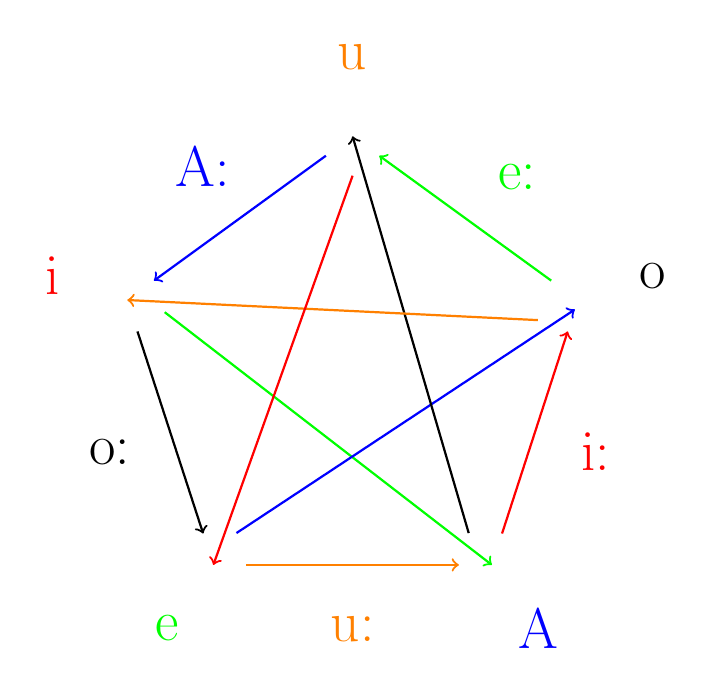
\begin{tikzpicture}

\node[regular polygon, minimum size = 8cm] (p) at (0,0) {};
\node[regular polygon, minimum size = 6cm] (q) at (0,0) {};
\node[regular polygon, minimum size = 5cm] (r) at (0,0) {};

\huge

\node[red] at (p.162){ i};
\node[orange] at (p.90) {u};
\node[green] at (p.234){e};
\node[blue] at (p.306) {\textipa{A}};
\node[black] at (p.378){o};

\node[blue] at (p.126){ \textipa{A:}};
\node[black] at (p.198){ \textipa{o:}};
\node[orange] at (p.270){ \textipa{u:}};
\node[red] at (p.342){ \textipa{i:}};
\node[green] at (p.50){ \textipa{e:}};

\draw[green, thick, ->] (r.162) -- (q.306);
\draw[blue,  thick, ->] ( r.234) -- (q.376);
\draw[black, thick, ->] (r.306) -- (q.90);
\draw[orange, thick, ->] (r.376) -- (q.162);
\draw[ red, thick, ->] (r.90) -- (q.234);

\draw[blue, thick, ->] (q.97) -- (q.155);
\draw[black, thick, ->] (q.169) -- (q.227);
\draw[orange, thick, ->] (q.241) -- (q.299);
\draw[red, thick, ->] (q.313) -- (q.371);
\draw[green, thick, ->] (q.385) -- (q.83);





\end{tikzpicture}
\end{center}

\section{Participles}

\begin{center}
\begin{tabular}{l| c c}
  & \textbf{Form} & \textbf{Translation}\\
  \hline
  \textbf{Active Past:} & \textipa{vr\=a\.*xa} & ``That which has attacked''\\
  \textbf{Passive Past:} & \textipa{avr\=a\.*xa} &  ``That which has previously been attacked''\\
  \textbf{Active Nonpast:} & \textipa{vr\=axka} & ``Fighting, battling''\\
  \textbf{Passive Nonpast:} & \textipa{avr\=axka} & ``Being attacked, under attack, besieged ''\\
  \hline
  \textbf{Active Future Past:} & \textipa{vreo\.*xe} & ``That which shall have attacked''\\
  \textbf{Passive Future Past:} & \textipa{avreo\.*xe} & ``That which shall have been attacked'' \\
  \textbf{Active Future Nonpast:} & \textipa{vreoxke} & ``That which shall attack'' \\
  \textbf{Passive Future Nonpast:} & \textipa{avreoxke} & ``That which shall be attacked'' \\


\end{tabular}

\end{center}

\end{document}
